\chapter{Ranking}

\section{Multiclass vs Multilabel}
Remember: multiclass classification is assigning a discrete label to a number of examples. 

For multiclass, each example has one and exactly one label, whereas with multilabel each example has 
{\bf zero} or multiple labels. \\
Some applications are: 
\begin{itemize}
	\item Reidentification
	\item Medical diagnosis
	\item Image annotation
\end{itemize}

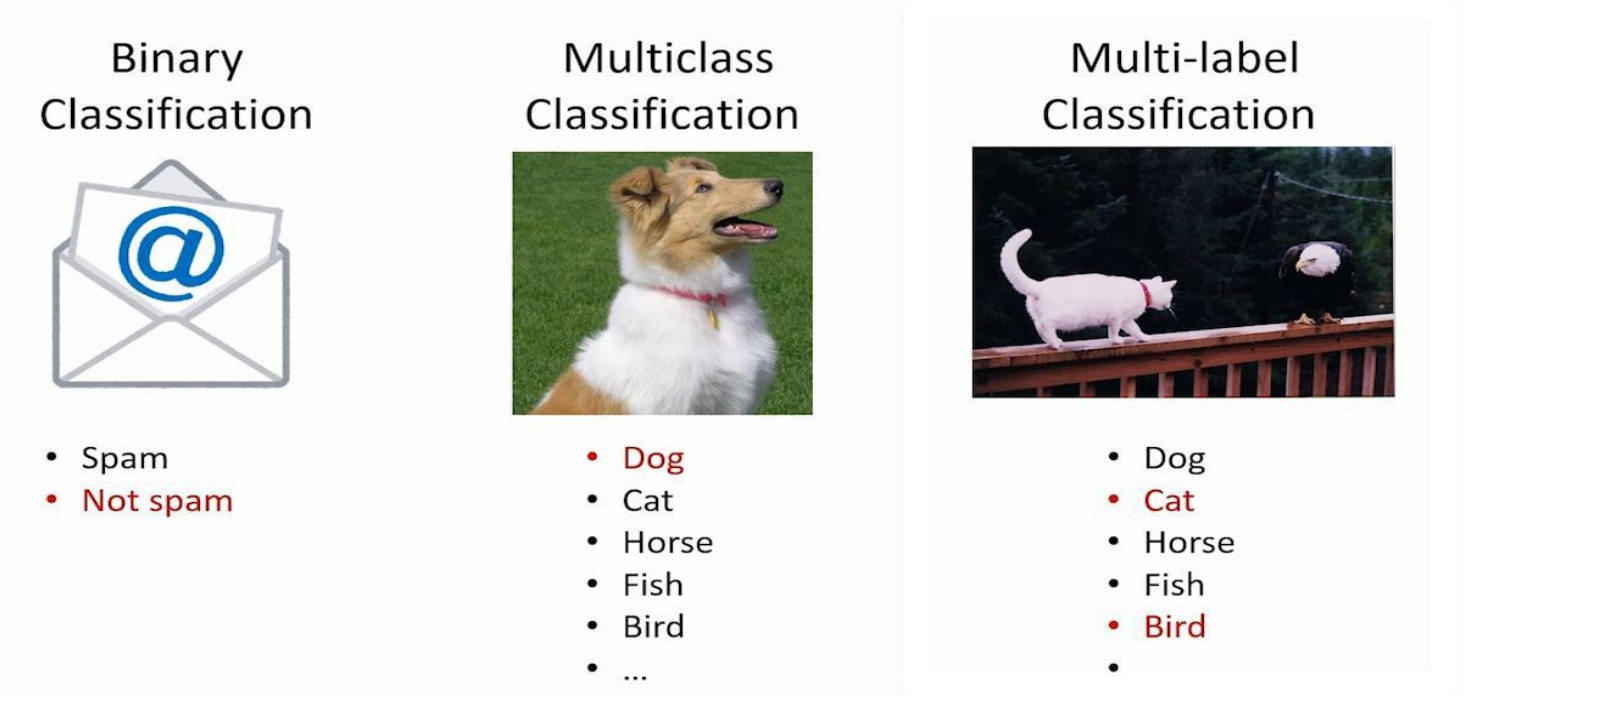
\includegraphics[scale=0.2]{classes}
\newpage
\section{Ranking}
In general the training data consists of a set of ranked examples. The {\bf ranker} will have to rank and order the test data. \\
Applications:
\begin{itemize}
	\item google search
	\item favourite movies
	\item loop closing in robotics
\end{itemize}

An approach could be using a binary classifier on pairings of examples and predict the better and worse between the two. The problem with this is that binary classifiers only take one example at the time.\\
The solution to this is to turn any pairings into one, comparing their features: 
\begin{equation}
	\begin{cases}
	1 & a_i \geq b_i \\
	0 & otherwise
	\end{cases}
\end{equation}
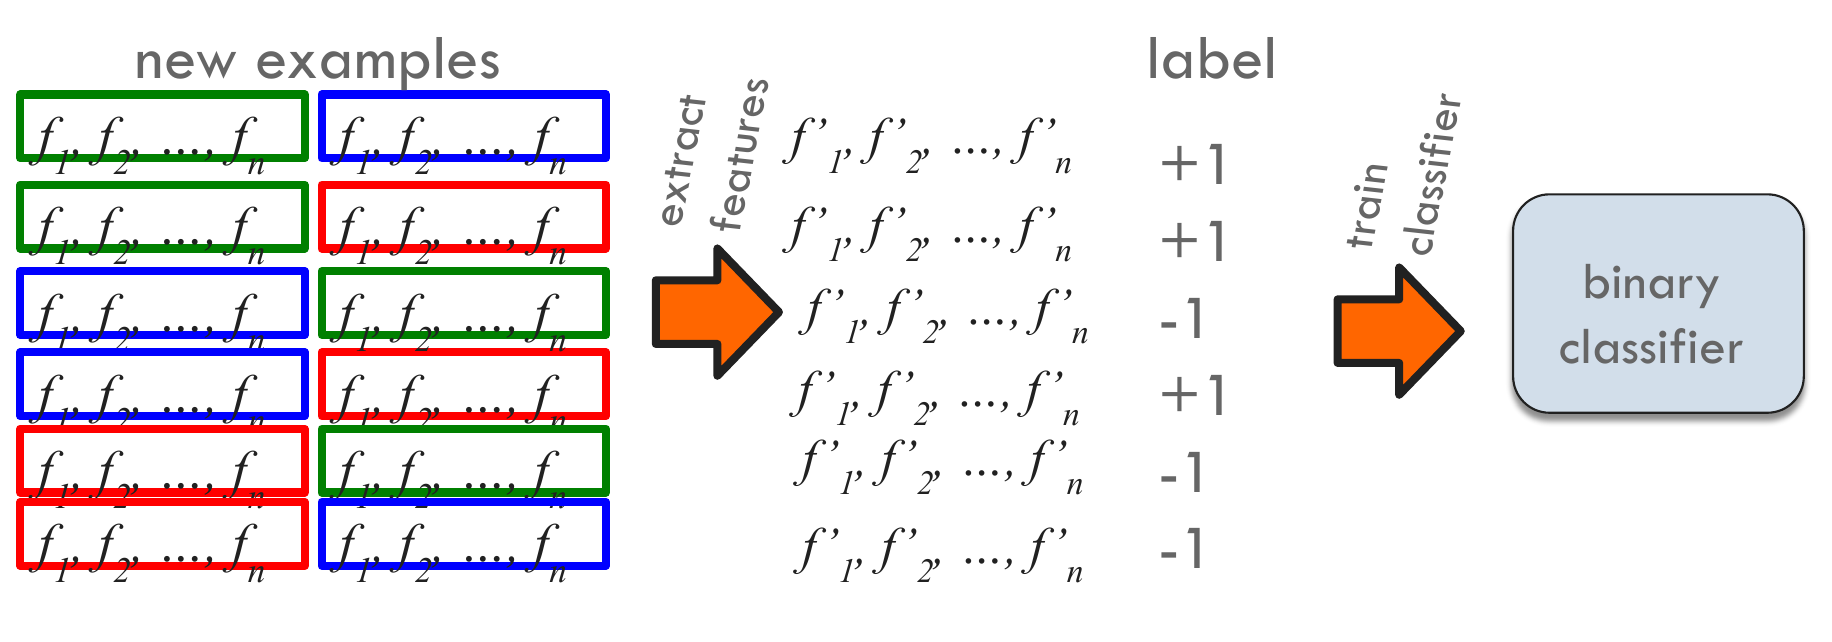
\includegraphics[scale=0.2]{ranking}

The final part of this algorithm is how to actually rank them and that's pretty straightforward: the ranking score will be equal to the sum of the rankings in the pairings. 

An application of this is if a document is relevant or not and in this case we would use a bipartite ranking system which is more similar to binary classification: is this document relevant or not? 
